\documentclass{article}

\usepackage[hidelinks]{hyperref}
\usepackage{graphicx}
\usepackage{titling}
\usepackage{float}
\usepackage[text={18cm,21cm},centering]{geometry}

\begin{document}

\begin{titlepage}
    \centering
    {\bfseries\LARGE Universidad de La Habana \par}
    \vspace{1cm}
    {\scshape\Large Facultad de Matemática y Computación \par}
    \vspace{3cm}
    {\scshape\Huge Simulación de eventos discretos (Inventario) \par}
    \vfill

    {\Large Pablo Gómez Vidal C-311 \par}
    
\end{titlepage}

\section*{Introducción}
Un proyecto de simulación de eventos discretos se enfoca en modelar y simular sistemas donde los cambios ocurren en momentos específicos en el tiempo, llamados "eventos discretos". Este tipo de simulación es útil para analizar sistemas complejos donde los procesos interactúan de manera no continua, como redes de comunicación, sistemas de colas, procesos de fabricación, o en el caso específico de este trabajo, la gestión de un inventario.
A través de este trabajo, se busca aplicar los principios de la simulación de eventos discretos para modelar
y experimentar con estos fenómenos, y obtener resultados que ayuden a tomar decisiones informadas.


\subsection*{Objetivos y metas}
\begin{enumerate}
    \item Desarrollar un sistema que permita modelar el problema
    \item Utilizar sus resultados para hacer un análisis estádistico a partir de estos, y a partir de dichos análisis tomar decisiones más informadas.
\end{enumerate}

\subsection*{Sistema a simular, el Inventario}


Para satisfacer las demandas, un dependiente debe mantener una cantidad del producto a mano, y siempre que el inventario a
mano se vuelve bajo, se ordenan unidades adicionales al distribuidor. Se utiliza una política de pedido (s, S); siempre que el inventario a mano es menor que $s$ y no hay un pedido pendiente, entonces se ordena una cantidad para llevarlo hasta $S$, donde $s<S$. Es decir, si el nivel de inventario actual es $x$ y no hay un
pedido pendiente, entonces si $x<s$ se ordena la cantidad $S-x$.
El costo de pedir y unidades del producto es una función especificada $c(y)$, y toma $L$ unidades de tiempo hasta que se
entrega el pedido, con el pago realizado a la entrega. Además, la tienda paga un costo de mantenimiento de inventario de
$h$ por unidad de artículo por unidad de tiempo,llámese mantenimiento de los productos.
Supongamos además que siempre que un cliente demanda más del producto de lo que está disponible actualmente, entonces se
vende la cantidad a mano y el resto del pedido se pierde para la tienda, esto no representa una pérdida real de dinero para la tienda, pero si una pérdida de una potencial venta.

El tendero está interesado en determinar el costo total esperado por unidad de tiempo para satisfacer la demanda del
producto:


\begin{itemize}

    \item Parámetros del sistema:
    \begin{itemize}
        \item  Tiempo máximo de la simulación ($t_{max}$).
        \item  Distribución del tiempo entre llegadas de los clientes ($T$).
        \item  Distribución de la demanda de los clientes para cada producto ($G$).
        \item  $s$, $S$, $L$, $h$, $c(y)$ para cada producto, $s$ es el nivel mínimo que debe alcanzar el producto, $S$ es el nivel máximo que debe alcanzar el producto, $L$ es el tiempo que toma en llegar el pedido del producto, $h$ es el costo de mantenimiento de inventario por unidad de artículo por unidad de tiempo, $c(y)$ es el costo de pedir y unidades del producto.
        \item Cantidad inicial de inventario ($I_0$).
        \item Cantidad inicial de dinero ($M_0$).
     \end{itemize}


    \item Variables de interés:
    \begin{itemize}
        \item Costo total esperado por unidad de tiempo para satisfacer la demanda del producto
        \item Valores de $s$ y $S$ que maximicen nuestra ganancia
    \end{itemize}
\end{itemize}


\section*{Detalles de la implementación}

En el directorio source se encuentran los archivos que contienen el código fuente de la simulación. 

El archivo \textbf{core.py}  contiene una abstractación de la simulación, en el se define lo que representa un \textbf{State}, un \textbf{Event}, \textbf{ApplyTimeEffects} y una función \textbf{simulation}

\begin{itemize}
    \item La clase \textbf{Event} representa un evento en la simulación. Cada evento tiene un tiempo asociado y una función \textbf{action} que ejecuta el evento.
    \item La clase \textbf{State} representa el estado de la simulación.
    \item La clase \textbf{ApplyTimeEffects} representa una acción que se ejecutará antes de cada evento programado.
    \item La función \textbf{simulation} que recibe como parámetros una cola con prioridad de eventos, una instancia de \textbf{ApplyTimeEffects},
  el estado
  inicial de la simulación, el tiempo máximo de la simulación y una función que determina si la simulación debe
  detenerse. La función ejecuta la simulación de la siguiente manera:
  Mientras haya eventos en la cola, se extrae el primer evento, si el tiempo del evento es menor o igual al tiempo
  máximo de la simulación, se ejecuta la acción de \textbf{ApplyTimeEffects}, luego se revisa si se cumple el caso de parada, en caso
  negativo se ejecuta el evento y se actualiza el estado de la simulación, y se vuelve a revisar si se cumple el caso de
  parada con este nuevo estado.
\end{itemize}
\end{itemize}

En \textbf{inventory.py} encontramos:

\begin{itemize}
    \item La clase \textbf{InventoryState} representa el estado del inventario.
    \item La clase \textbf{RefillInventoryEvent} representa el evento de reabastecimiento del inventario.
    \item La clase \textbf{SaleProductEvent} representa el evento de venta de un producto.
    \item La clase \textbf{InventoryConfig} representa la configuración del inventario.
    \item La clase \textbf{ApplyTimeEffectsInventory} representa la característica de nuestro problema de pagar el costo de
  mantenimiento de inventario por unidad de artículo por unidad de tiempo.
\end{itemize}

En \textbf{simulation.py} se define:

\begin{itemize}
    \item La función \textbf{inventory\_simulation} que recibe como parámetros el tiempo máximo de la simulación, la distribución del
  tiempo entre llegadas de los clientes, la lista con configuraciones del inventario, la distribución de la demanda de
  los clientes
  para cada producto, la cantidad inicial de cada producto en el inventario, la cantidad inicial de dinero y una función
  que determina si
  la simulación debe detenerse.
  La función inicializa el estado de la simulación, crea la cola con prioridad de eventos y ejecuta la
  simulación descrita en el módulo anterior.


\section*{Resultados y Experimentos}

Pensemos que gestionamos una tienda que vende un solo producto, y nuestro objetivo es comparar diferentes combinaciones de los parámetros s y S con el fin de maximizar la ganancia promedio obtenida durante una semana.

\vspace{\baselineskip}

El análisis y desarrollo se encuentra en analitics.ipynb.

\vspace{\baselineskip}

Nuestro modelo tiene esta forma:
\begin{itemize}
    \item Unidad de tiempo: hora
    \item  Tiempo máximo de la simulación $t_{max} = 24 \cdot 7$.
    \item  Distribución del tiempo entre llegadas de los clientes $T \sim Exp(\beta = 8)$.
    \item  Distribución de la demanda de los clientes para el producto $D \sim U(1,5)$.
    \item Unidades de tiempo que toma en llegar el pedido del producto $L = 4$
    \item Costo de mantenimiento de inventario por unidad de artículo por unidad de tiempo $h=1/100$
    \item Costo de pedir y unidades del producto $c(y) = y \cdot 50$
    \item Precio al que se vende una unidad de producto $p = 100$
    \item Cantidad inicial de inventario $I_0 = S$. Inicialicemos el almacén lleno.
    \item Cantidad inicial de dinero $M_0 = 0$.
\end{itemize}

Probemos diferentes valores de $s$ y $S$:
\begin{itemize}
    \item Nivel mínimo que debe alcanzar el producto $s = 30$
    \item Nivel máximo que puede haber de producto en el almacén i:
    $S_1 = 80$ y $S_2 = 100$
\end{itemize}

Comparemos ambos sistemas

\vspace{\baselineskip}

Hagamos 100 simulaciones en cada uno, quédandonos con el dinero con el que terminaron en cada simulación, hallemos las medias para cada sistema y vamos a compararlas. A continuación los resultados:
\begin{enumerate}
    \item La media del sistema con {S=100} fue aproximadamente 4653.72 con una desviación estándar de 1493.62.
    \item La media del sistema con {S=80} fue aproximadamente 3218.87 con una desviación estandar de 1914.51
\end{enumerate}

A continuación podemos visualizar los datos de ambas políticas:

\begin{figure}[H]
    \centering
    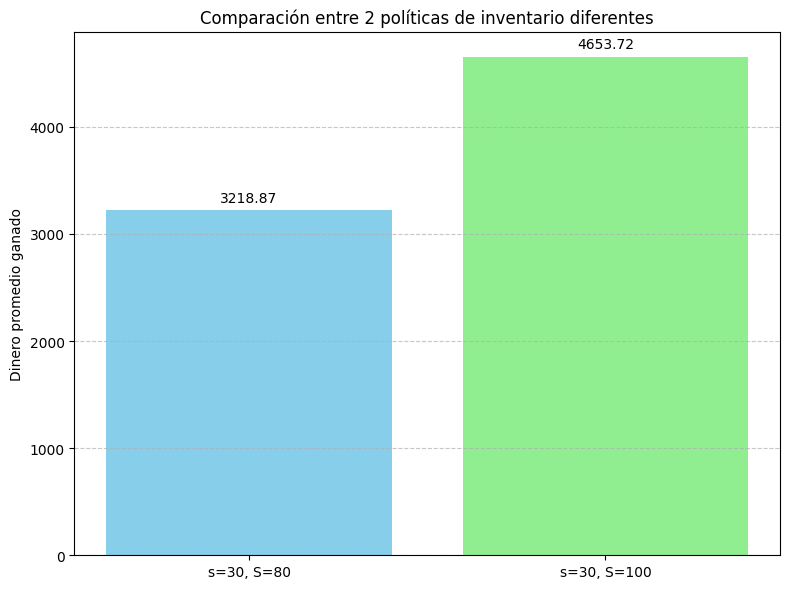
\includegraphics[width=0.7\linewidth]{./output1.png}
    \label{fig:enter-label}
\end{figure}

Tanto en el gráfico como en los datos pudimos observar que se obtuvo mejores resultados con $S = 100$, o sea teniendo un almacén más grande.\\

\section*{Prueba de hipótesis para comparar políticas de inventario}

\subsection*{Objetivo}

Evaluar si existe una diferencia significativa en el rendimiento económico entre dos políticas de inventario, definidas por distintos parámetros $(s, S)$, al finalizar un periodo simulado. El rendimiento se mide en términos del dinero total acumulado al final de cada simulación.

\subsection*{Hipótesis}

Se plantean las siguientes hipótesis estadísticas sobre la diferencia de medias:

\begin{itemize}
    \item \textbf{Hipótesis nula} ($H_0$): No existe diferencia en el rendimiento medio entre ambas políticas.\\
    $H_0: \mu_1 - \mu_2 = 0$
    
    \item \textbf{Hipótesis alternativa} ($H_1$): Existe una diferencia significativa en el rendimiento medio.\\
    $H_1: \mu_1 - \mu_2 \ne 0$
\end{itemize}

\subsection*{Método: Bootstrap para la diferencia de medias}

Dado que los resultados de la simulación no siguen una distribución normal, (dato que se demuestra en el analitics.ipynb) se utiliza un enfoque no paramétrico mediante el método \textit{Bootstrap}:

\begin{enumerate}
    \item Se calcula la diferencia observada entre las medias de ambas simulaciones:
    \[
    \bar{X}_{\text{diff}} = \bar{X}_1 - \bar{X}_2
    \]
    
    \item Se generan múltiples muestras \textit{bootstrap} (por ejemplo, $10\,000$), re-muestreando con reemplazo de los datos originales de cada simulación.
    
    \item Para cada par de muestras \textit{bootstrap}, se calcula la diferencia de medias.
    
    \item Se construye un intervalo de confianza del $95\%$ a partir de los percentiles $2.5$ y $97.5$ de las diferencias bootstrap:
    \[
    IC_{95\%} = \left[P_{2.5}(\Delta \bar{X}),\; P_{97.5}(\Delta \bar{X})\right]
    \]
\end{enumerate}

\subsection*{Criterio de decisión}

\begin{itemize}
    \item Si $0 \in IC_{95\%}$, no se rechaza la hipótesis nula. No hay evidencia estadísticamente significativa de diferencia entre las políticas.
    \item Si $0 \notin IC_{95\%}$, se rechaza $H_0$. Existe evidencia de una diferencia estadísticamente significativa entre las políticas.
\end{itemize}

En nuestro caso el intervalo de confianza hallado fue de [$-1936.22$, $-1085.99$]
por lo que existe una diferencia estadísticamente significativa entre las políticas usadas en ambas simualciones.

\begin{figure}[H]
    \centering
    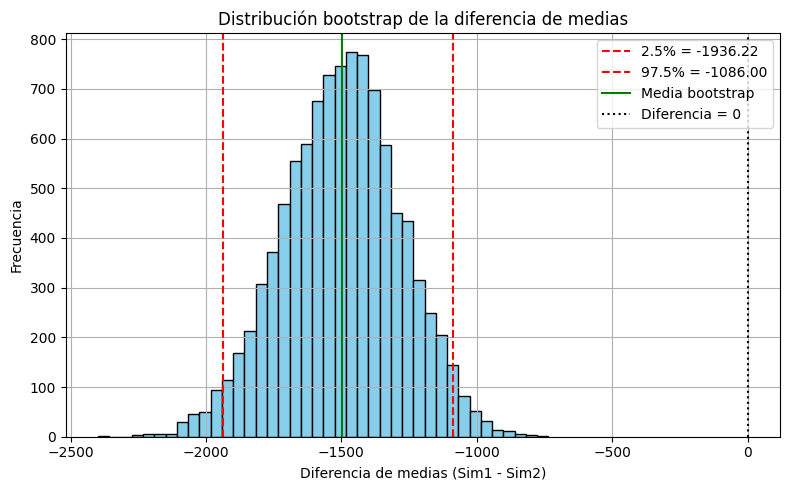
\includegraphics[width=0.7\linewidth]{./output2.png}
    \label{fig:enter-label}
\end{figure}

\section*{Modelo matemático}
Este modelo matemático permite la simulación de un inventario de un establecimiento en los que los clientes llegan (definiendo intervalos de tiempo que distribuyen exponencial) y demandan cierto producto, esta demanda se rige por una variable aleatoria con distribución $G$. Si actualmente en el inventario no se dispone de la cantidad demandada por el cliente este realiza la compra de lo que quede, en caso contrario se efectúa la compra de la cantidad que demanda el cliente y se resta esa demanda a la cantidad del inventario. El abastecimiento del establecimiento se rige por una política $s$ - $S$, si el inventario se disminuye su volumen por debajo de $s$ se solicita un reabastecimiento de $S-k$ unidades donde $k$ es el volumen actual del inventario. Dicho reabastecimiento tiene un consto definido por una función $c(y)$ y demora $L$ unidades de tiempo. Además se paga por almacenamiento de los productos en el inventario definido por $h*k*i$ donde $i$ representa el intervalo de tiempo y $k$ el volumen del inventario durante ese período.

\subsection*{Descripción}

\subsection*{Variables implicadas en el modelo}

\begin{itemize}
    \item $t$ tiempo actual.
    \item $t_q$ tiempo asociado al evento que determina la llegada de un cliente.
    \item $t_y$ tiempo asociado al evento que determina un reabastecimiento.
    \item $k$ volumen del inventario.
    \item $x$ presupuesto actual.
    \item $y$ cantidad de volumen del reabastecimiento.
    \item $l$ tiempo que demora el reabastecimiento.
    \item $h$ costo por unidad de tiempo.
    \item $p$ precio de una unidad del producto.
\end{itemize}

\subsection*{Valores iniciales}

\begin{itemize}
    \item $t=0$.
    \item $t_q=q$ donde $q$ es una variable que distribuye exponencial.
    \item $t_y$ parámetro de la simulación.
    \item $k=S$.
    \item $x=0$.
    \item $y=0$.
    \item $l=4$.
    \item $h=1/100$ .
    \item $p=100$.
\end{itemize}

\subsection*{Eventos}

\begin{enumerate}
    \item Llegada de un cliente: se actualiza $t=t_q$. Se genera una variable aleatoria $w$ con distribución $G$, si $w>k$, $k=0$ y $x=x+p(k)$, en caso contrario $k=k-w$ y $x=x+p(w)$. Si $k<s$ se genera un evento reabastecimiento con $t_y=t+l$ y $y=S-k$. Dejar $t_q=t+q$ donde $q$ es una variable que distribuye exponencial (para analizar la próxima llegada).
    \item Llegada de un reabasteciemiento: se actualiza $t=t_y$. Se actualiza $k=k+y$ y $x=x-c(y)$.
    \item Calcular el costo de almacenamiento: se actualiza $x=x-h*i*k$.
\end{enumerate}

\subsection*{Supuestos y restricciones}

\begin{itemize}
    \item $c(y)$ costo del reabastecimiento de y unidades del producto.
    \item  Distribución del tiempo entre llegadas de los clientes $T \sim Exp(\beta = 8)$.
    \item  Distribución de la demanda de los clientes para el producto $G \sim U(1,5)$.
    \item  El evento de calcular el costo de almacenamiento ocurre antes de realizarse cada uno de los restantes eventos y luego de terminar la simulación.

\end{itemize}

\section*{Conclusiones}

\begin{itemize}
    \item \textbf{Comparación efectiva de políticas:} La simulación permitió comparar el desempeño de dos políticas de reabastecimiento tipo \((s, S)\), evaluando su impacto sobre el beneficio económico final. Esta metodología fue clave para tomar decisiones informadas sin necesidad de aplicar el sistema en un entorno real.

    \item \textbf{Evaluación basada en dinero final:} La variable principal evaluada fue el dinero acumulado al finalizar el periodo simulado, lo cual refleja de forma directa la eficiencia de cada política de inventario, considerando costos de reabastecimiento, costos de almacenamiento y ventas efectivas.

    \item \textbf{Validez estadística mediante intervalos de confianza:} Se construyeron intervalos de confianza al 95\% para el dinero promedio final de cada simulación. La comparación de estos intervalos ofreció una primera aproximación al análisis de significancia de las diferencias entre políticas.

    \item \textbf{Análisis de la diferencia y prueba de hipótesis:} Se estimó el intervalo de confianza para la diferencia entre los promedios usando tanto inferencia clásica como el método bootstrap. En ambos casos, se concluyó que la diferencia observada es estadísticamente significativa, ya que el intervalo de confianza no incluía el cero.




\end{document}